\subsubsection{Text preprocessing}
\label{sub:text_preprocessing}

\outline{Neural networks only require inputs to be numbers (vectors or scalars)}
\outline{Need to translate text into numbers, i.e., obtain vector representation for words}
\outline{This is called an embedding (layer)}
\outline{Section will use simple example for preprocessing steps, but also
describe intermediate results for collected data sets}
\outline{Introduce simple example: texts}

\paragraph{Word vectors}
\label{sub:word_vectors}

\outline{Basic concept: words are transformed into vectors with dimensionality d}
\outline{This places words in a vector space}
\outline{Allows examination of space structure and relationships between words}

\outline{Thesis uses pre-trained word vectors: GloVe (NLP Stanford)}
\outline{Trained on 2B tweets containing 27B unique tokens from different languages (English, Arabic, Japanese)}
\outline{Vectors are obtained by examining co-occurrence statistics in given data}
\outline{Token can be a word or symbol with special meaning, e.g., tokens for numbers, punctuation repetition}
\outline{Special features of these pretrained vectors: nearest neighbors, linear substructures} 
\outline{Nearest neighbors: possibility to use Euclidian distance to quantify
linguistic or semantic similarity between words}
\outline{Linear substructures: calculating semantic distance allows to compare
relatedness, e.g., man <=> woman similar to king <=> queen (underlying concept to distinguish is gender)}

\paragraph{Tokenization}
\label{sub:tokenization}

\outline{Raw tweet texts need to adapt to chosen word vectors}
\outline{Most importantly: use predefined tokens in order to get the maximum
benefit out of pretrained word vectors}
\outline{Goal: Text should be able to be separated into tokens by simply splitting on spaces}

\begin{table}
\begin{tabular}{rlll}
\toprule
Step & Description & Before & After \\
\midrule
1 & Mark URLs & ``https://t.co/IFt05'' & ``<url>'' \\
2 & Split words separated by slashes & ``fruits/vegetables'' & ``fruits / vegetables'' \\
3 & Mark user mentions & ``@rogerfederer'' & ``<user>'' \\
4 & Mark emoticons & ``:-)'' & ``<smile>'' \\
5 & Mark numbers & ``123'' & ``<number>'' \\
6 & Mark and split hashtags & ``\#SoNice'' & ``<hashtag> so nice'' \\
7 & Mark punctuation repetitions & ``!!!'' & ``! <repeat>'' \\
8 & Add spaces around punctuation & ``Watch out!'' & ``watch out !'' \\
9 & Mark elongated words & ``niceeeee'' & ``nice <elong>'' \\
10 & Mark allcaps words & ``IMPORTANT'' & ``important <allcaps>'' \\
11 & Remove unicode character & ``u00B3'' & `` '' \\
\bottomrule
\end{tabular}
\caption{Order of text preprocessing steps}
\label{tab:text_preprocessing}
\end{table}

\begin{figure}[h]
  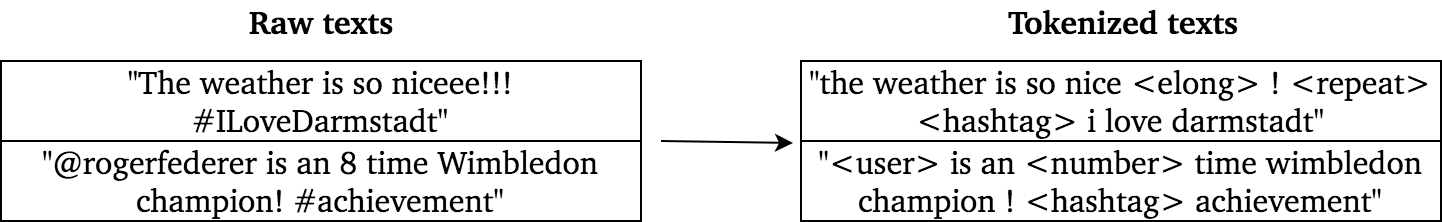
\includegraphics[width=\textwidth]{img/text_preprocessing_1}
  \caption{Tokenization example}
\label{fig:tokenization}
\end{figure}

\outline{List of steps inspired by provided Ruby scripts, but fixed and expanded}
\outline{Step 1: Replace URLs => only occurrence is notable, extracting meaning very difficult}
\outline{Step 2: Split words separated by slashes => get singular words}
\outline{Step 3: Replace user mentions => same as URLs}
\outline{Step 4: Replace specific emojis => could be sign of sentiment}
\outline{Step 5: Replace numbers => sames as URLs}
\outline{Step 6: Split hashtags on uppercase letters => derive their meaning}
\outline{Step 7: Mark punctuation repetitions => mark importance of sentiment}
\outline{Step 8: Add spaces around punctuation => separate from words}
\outline{Step 9: Mark elongated words => possible sign of exaggeration}
\outline{Step 10: Mark allcaps words => possible sign of exaggeration}
\outline{Step 11: Replace unicode characters => avoid preprocessing errors}

\outline{Example: apply tokenization to example texts}

\paragraph{Word index}
\label{sub:word_index}

\begin{figure}[h]
  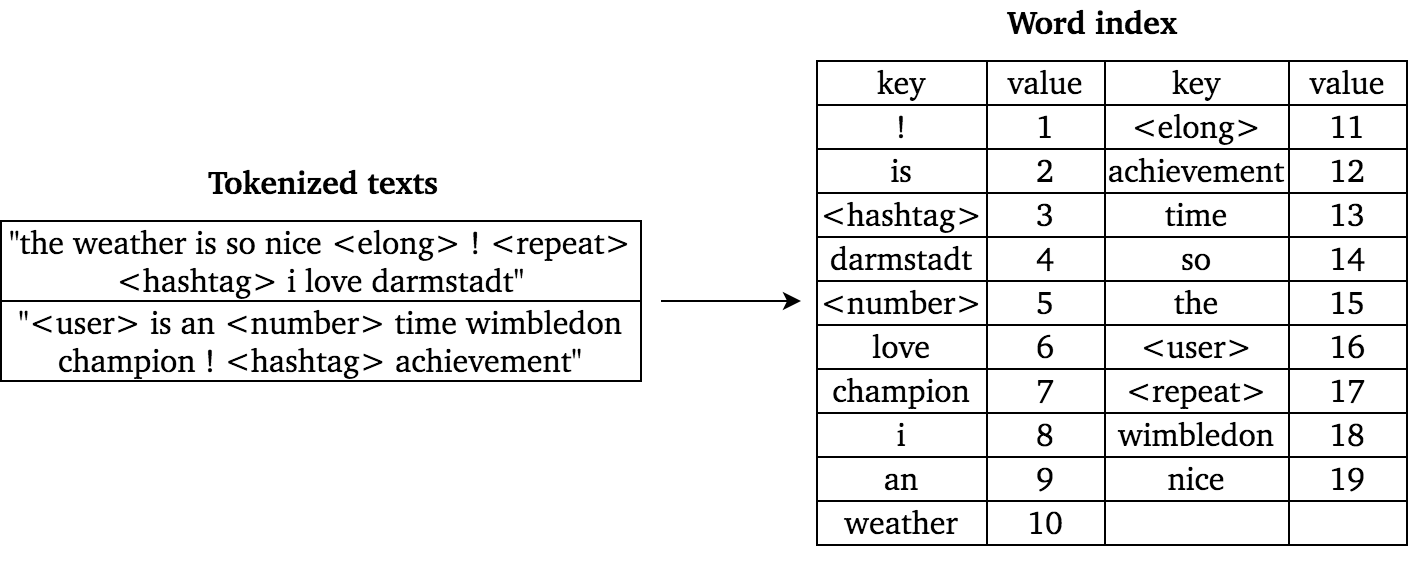
\includegraphics[width=\textwidth]{img/text_preprocessing_2}
  \caption{Word index example}
\label{fig:word_index}
\end{figure}

\outline{First step of embedding creation: get a list of all occurring words}
\outline{Word index: map (key => word, value => unique ID)}
\outline{IDs are usually ordered by number of occurrences, s.th. most important
words can be extracted if number of words is limited for some reason}
\outline{List number of words for data sets + most common words}
\outline{Important: IDs are ascending (step size 1) and start 1}

\paragraph{Sequences}
\label{sub:sequences}

\begin{figure}[h]
  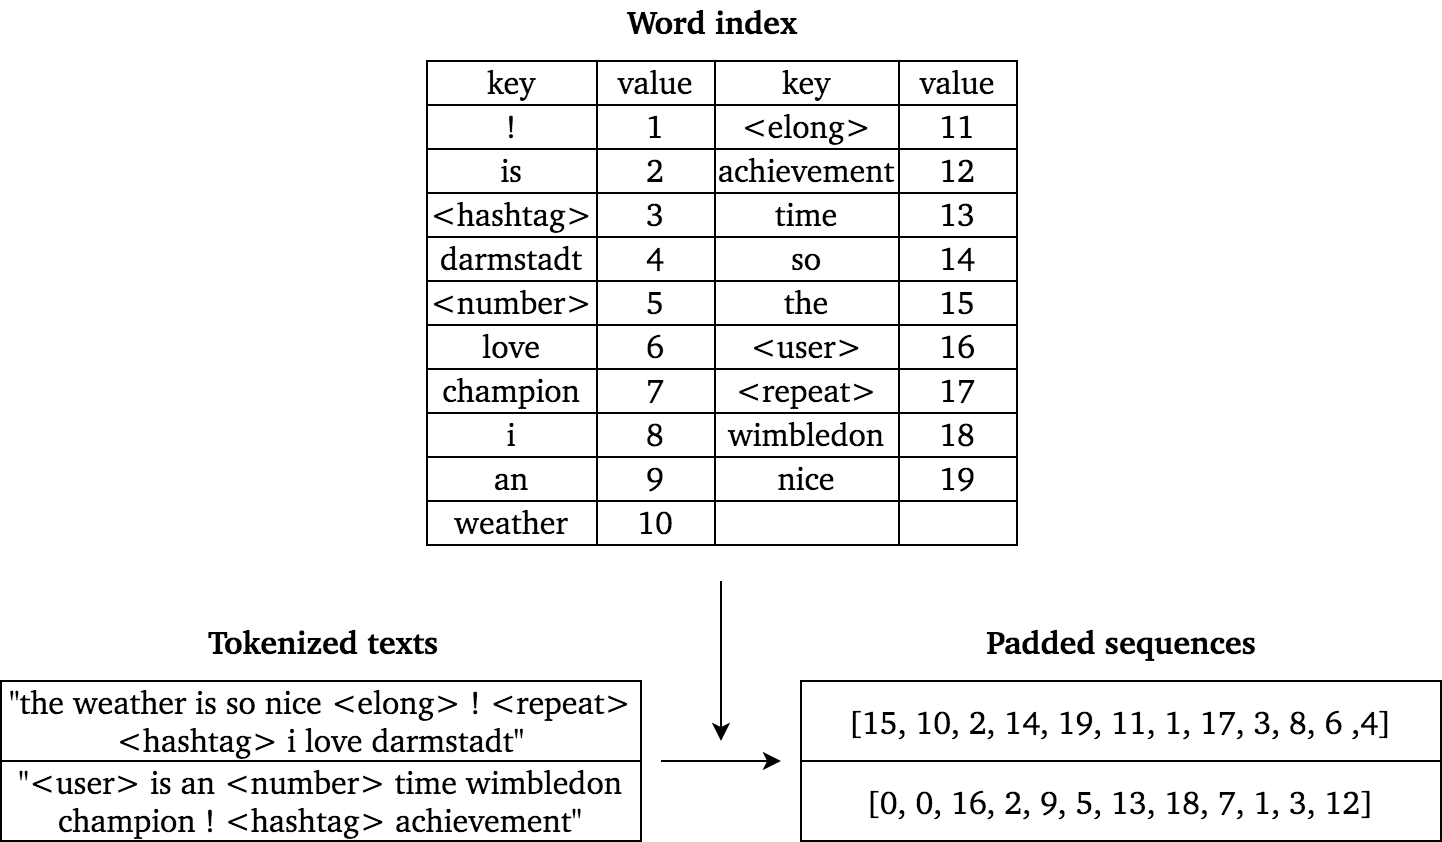
\includegraphics[width=\textwidth]{img/text_preprocessing_3}
  \caption{Text sequencing example}
\label{fig:text_sequencing}
\end{figure}

\outline{Second step: transform texts into sequence (i.e., list of word IDs)}
\outline{Split on whitespace (space, tab, newline)}
\outline{Lookup word ID in word index}
\outline{Zero-pad sequences according to specification (e.g., longest sequence)}

\paragraph{Embedding index}
\label{sub:embedding_index}

\begin{figure}[h]
  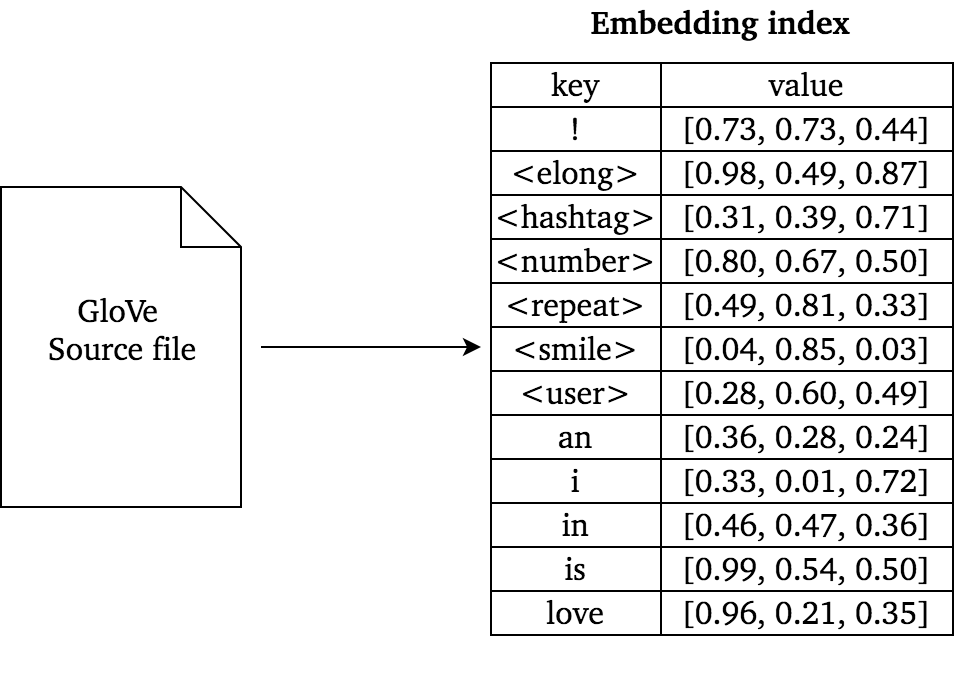
\includegraphics[height=7cm]{img/text_preprocessing_4}
  \caption{Embedding index example}
\label{fig:embedding_index}
\end{figure}

\outline{Third step: load pretrained word vectors from file}
\outline{Create a map (key: word, value: d-dimensional vector)}

\paragraph{Embedding matrix}
\label{sub:embedding_matrix}

\begin{figure}[h]
  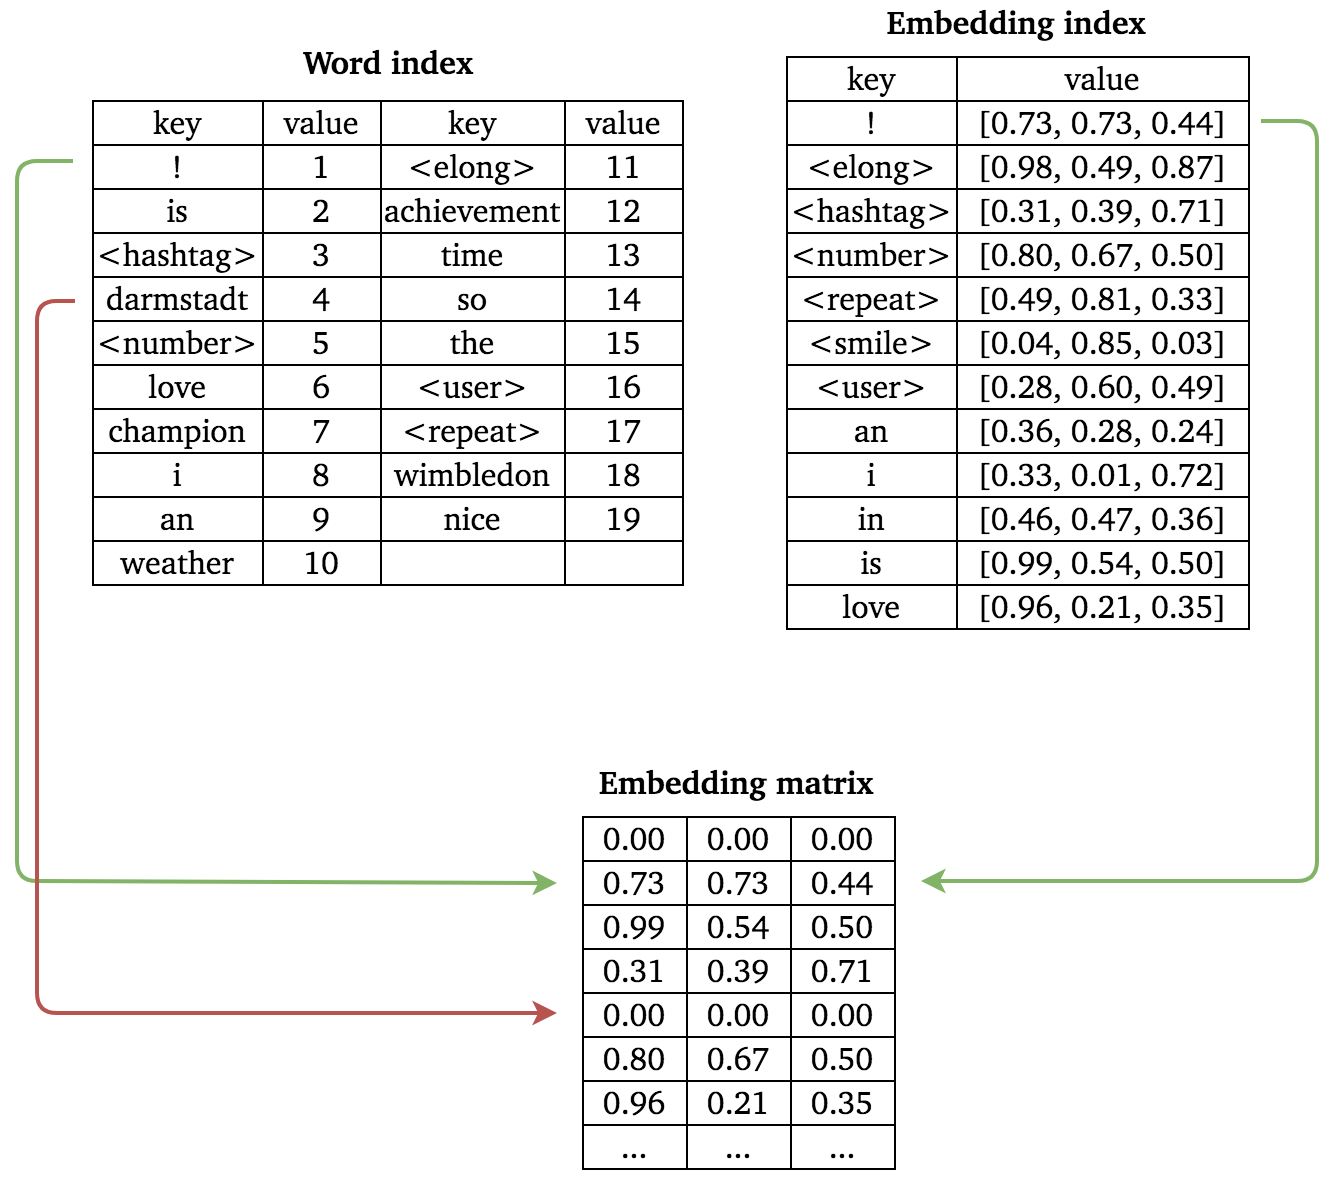
\includegraphics[width=\textwidth]{img/text_preprocessing_5}
  \caption{Embedding matrix example}
\label{fig:embedding_matrix}
\end{figure}

\outline{Final step: create a matrix in which the i-th row represents the word
vector for the word with ID i from word index}
\outline{Dimensionality: (number of words) x d}
\outline{Enables simple lookup procedure for the network}
\outline{Zero row is default for unknown words (i.e., words that were not found in pretrained
word vectors)}


